% mnras_template.tex 
%
% LaTeX template for creating an MNRAS paper
%
% v3.0 released 14 May 2015
% (version numbers match those of mnras.cls)
%
% Copyright (C) Royal Astronomical Society 2015
% Authors:
% Keith T. Smith (Royal Astronomical Society)

% Change log
%
% v3.0 May 2015
%    Renamed to match the new package name
%    Version number matches mnras.cls
%    A few minor tweaks to wording
% v1.0 September 2013
%    Beta testing only - never publicly released
%    First version: a simple (ish) template for creating an MNRAS paper

%%%%%%%%%%%%%%%%%%%%%%%%%%%%%%%%%%%%%%%%%%%%%%%%%%
% Basic setup. Most papers should leave these options alone.
\documentclass[fleqn,usenatbib]{mnras}

% MNRAS is set in Times font. If you don't have this installed (most LaTeX
% installations will be fine) or prefer the old Computer Modern fonts, comment
% out the following line
\usepackage{newtxtext,newtxmath}
% Depending on your LaTeX fonts installation, you might get better results with one of these:
%\usepackage{mathptmx}
%\usepackage{txfonts}

% Use vector fonts, so it zooms properly in on-screen viewing software
% Don't change these lines unless you know what you are doing
\usepackage[T1]{fontenc}

% Allow "Thomas van Noord" and "Simon de Laguarde" and alike to be sorted by "N" and "L" etc. in the bibliography.
% Write the name in the bibliography as "\VAN{Noord}{Van}{van} Noord, Thomas"
\DeclareRobustCommand{\VAN}[3]{#2}
\let\VANthebibliography\thebibliography
\def\thebibliography{\DeclareRobustCommand{\VAN}[3]{##3}\VANthebibliography}


%%%%% AUTHORS - PLACE YOUR OWN PACKAGES HERE %%%%%

% Only include extra packages if you really need them. Common packages are:
\usepackage{graphicx}	% Including figure files
\usepackage{amsmath}	% Advanced maths commands
\usepackage{float}

%%%%%%%%%%%%%%%%%%%%%%%%%%%%%%%%%%%%%%%%%%%%%%%%%%

%%%%% AUTHORS - PLACE YOUR OWN COMMANDS HERE %%%%%

% Please keep new commands to a minimum, and use \newcommand not \def to avoid
% overwriting existing commands. Example:
%\newcommand{\pcm}{\,cm$^{-2}$}	% per cm-squared

%%%%%%%%%%%%%%%%%%%%%%%%%%%%%%%%%%%%%%%%%%%%%%%%%%

%%%%%%%%%%%%%%%%%%% TITLE PAGE %%%%%%%%%%%%%%%%%%%

% Title of the paper, and the short title which is used in the headers.
% Keep the title short and informative.
\title[Population III IMF convergence: Sink Particle creation densities]{Population III IMF convergence: Sink Particle creation densities}

% The list of authors, and the short list which is used in the headers.
% If you need two or more lines of authors, add an extra line using \newauthor
\author[L. R. Prole]{
Lewis R. Prole,$^{1}$\thanks{E-mail: Prolel@cardiff.ac.uk}
Paul C. Clark,$^{2}$
$$
$$
\\
% List of institutions
$^{1}$Cardiff University School of Physics and Astronomy\\
$^{2}$Cardiff University School of Physics and Astronomy\\
$.$
}

% These dates will be filled out by the publisher
\date{Accepted XXX. Received YYY; in original form ZZZ}

% Enter the current year, for the copyright statements etc.
\pubyear{2020}

% Don't change these lines
%\hypersetup{draft}
\begin{document}

\label{firstpage}
\pagerange{\pageref{firstpage}--\pageref{lastpage}}
\maketitle

% Abstract of the paper
\begin{abstract}
The Population III initial mass function (IMF) is currently unknown, but recent studies agree that fragmentation of primordial gas gives a broader IMF than the initially accepted singular star per halo. Sink particles introduced at high densities can prevent artificial fragmentation of the gas once the mesh stops refining, but an incorrect choice of sink particle creation density will effect the resulting IMF. This study introduces sink mergers into AREPO, and presents the effects of varying the sink particle creation density from $\rho_{\text{sink}}$=10$^{-10}$-10$^{-6}$gcm$^{-3}$. Turbulent primordial cloud collapses were performed, resulting in periodic bursts of star formation. While the total mass accreted and accretion rates onto sinks were invariant to $\rho_{\text{sink}}$, the total number of sinks formed N$_{\text{sink}}$ increased with increasing $\rho_{\text{sink}}$, without converging within the range tested. The cooling time-scale of the gas becomes smaller than the free-fall time at $\sim 10^{-6}$gcm$^{-3}$, causing instability to fragmentation and an increased number of sinks forming when gas was allowed to collapse beyond this density. The number of sink ejections from the system also increased with increasing $\rho_{\text{sink}}$, owing to higher velocities resolved by the increased maximum resolution. Despite the non-convergence of N$_{\text{sink}}$, the IMF stops shifting towards lower masses when sinks are created at densities of 10$^{-7}$gcm$^{-3}$. As most previous Pop III studies involving sink particles have introduced sinks at lower densities than this, their resulting IMFs have overestimated the mass of primordial stars.
\end{abstract}

% Select between one and six entries from the list of approved keywords.
% Don't make up new ones.
\begin{keywords}
stars: Population III -- stars: formation -- hydrodynamics -- stars: luminosity function, mass function -- software: simulations
\end{keywords}

%%%%%%%%%%%%%%%%%%%%%%%%%%%%%%%%%%%%%%%%%%%%%%%%%%

%%%%%%%%%%%%%%%%% BODY OF PAPER %%%%%%%%%%%%%%%%%%

\section{Introduction}
The first stars, known as Population III (Pop III) stars, are responsible for the first ionising radiation, which began the epoch of re-ionisation \citep{Bromm2001}. When they died as supernovae, they injected the interstellar medium (ISM) with the first metals \citep{Heger2003}, which would go on to form the next generation (Pop II) of stars. During their formation, the primordial magnetic seed field was amplified via the small-scale magnetic dynamo (e.g. \citealt{Schober2012}), which may have been the first step in converting the small scale, chaotic primordial fields into the coherent, large scale galactic magnetic fields observed today \citep{Kulsrud1990}. Evidently the initial mass function (IMF) of Pop III stars has a huge effect on the evolution of the Universe. Initially it was thought that Pop III stars formed in isolation \citep{Haiman1996}, and were massive \citep{Bromm1999}, yet further studies showed they were susceptible to fragmentation in the presence of subsonic turbulence \citep{Clark2011}. Since then, numerical studies have attempted to improve the picture of Pop III star formation by including feedback mechanisms \citep{OShea2008}, live dark matter potentials \citep{Stacy2014} and magnetic fields (e.g. \citealt{Machida2008a}, \citealt{Sharda2020}). Despite this, the Pop III IMF is still in dispute, and there are still many factors left to study.

A limmiting factor in star formation simulations is minimum resoltuion. The Jeans length $\lambda_J$ of a structure of given density and temperature marks the maximum size it can achieve before thermal pressure cannot resist against gravitational collapse. Hence artificial fragmentation occurs in hydrodynamic codes if the local $\lambda_J$ falls below the size of mesh cells $\Delta x$. To prevent this, the mesh refines itself based on the local $\lambda_J$, which depends on the temperature and density of the gas. The Truelove condition \citep{Truelove1997} requires a Jeans number $\Delta x/\lambda_J$ of 0.25, corresponding to at least 4 cells spanning across any $\lambda_J$, to prevent artificial fragmentation. Numerical simulations cannot refine indefinitely; as the gas gets denser (decreasing $\lambda_J$), it becomes computationally expensive to refine further. Sink particles \citep{Bate1995} provide an alternative to indefinite refinement, they are non-gaseous particles that contain all of the mass within the area they occupy and can accrete matter from their surrounding cells. As they cannot fragment -either naturally or artificially- their implementation at high densities overcomes the Jeans refinement criteria. In present day star formation simulations, the sink creation density is chosen to be that of the first adiabatic core. As laid out in \cite{Larson1969}, the initial isothermal collapse of a cloud is halted in the central region when the gas becomes opaque to outgoing radiation and the energy is absorbed into the star. At $\sim$10$^{-10}$gcm$^{-3}$, the central temperature and density are such that collapse halts in the central region, forming the first adiabatic core, while the material outside the core continues to freefall isothermally. At this point the core is stable to further fragmentation. The radial density profile inside the core is flat and extends out to $\lambda_J$, so the radius of the of sink particle is chosen to be the Jeans length at the creation density and temperature. In primordial star formation, there is no clear 'first core', the thermal evolution is described in \cite{Omukai2005}. Saturation of the H$_2$ cooling rate at 10$^{-20}$gcm$^{-3}$ allows the gas temperature to rise from 200K to 1000K by 10$^{-15}$gcm$^{-3}$. Here three-body reactions convert most of the hydrogen into molecules. At 10$^{-12}$gcm$^{-3}$, the H$_2$ cooling rate decreases due to  gas opacity, but collision-induced emission kicks in to become the dominant cooling process at 10$^{-10}$gcm$^{-3}$. Once the temperature reaches 2000K at 10$^{-9}$gcm$^{-3}$, dissociation of H$_2$ molecules provides effective cooling until it is depleted and the collapse becomes almost adiabatic at 10$^{-4}$gcm$^{-3}$. Running simulations up to this density with a full chemical treatement lies beyond current computational capabilities. Hence, the appropriate time to replace gas with a stable sink particle is unclear. \cite{Smith2011} studied the stability of Pop III collapses against fragmentation during the early period of protostar formation, before ionizing radiation from the star becomes important, where accretion luminocity feedback is the main opposition to fragmentation. They found that accretion luminosity delays fragmentation but doesn’t prevent it. \cite{Gammie2001} suggested that disks become stable to fragmentation when heating from turbulence is balaced by cooling. However, \cite{Meru2011} showed that the critical cooling time needed for stability increases with resolution, hence fragmentation is resolution dependent. This suggests that the Gammie criterion does not indicate if a disk is stable. The sink particle creation density varies across authors e.g. \cite{Clark2011} and \cite{Sharda2020} introduce sinks at $\sim$10$^{-11}$gcm$^{-3}$ in analogy with present day star formation, while \cite{Smith2011} and \cite{Wollenberg2019} introduce them at $\sim$10$^{-9}$gcm$^{-3}$, above which there are no chemical heating terms that can prevent the gas from collapsing. Sink particles are not a perfect solution to the indefinite refinement problem, and an authors choice of sink particle creation density will change the morphology of the resulting cluster. This paper explores the effect of varying the sink particle creation density from 10$^{-10}$ - 10$^{-6}$gcm$^{-3}$, within the frame of primordial Pop III gas collapse. The most important parameters to track are the total number of sinks formed and the total combined mass of the sinks.



\section{Sink parameters}

The radius of a sink particle is chosen to be $\lambda_J$ corresponding to the sink creation density, given by


\begin{equation}
    \lambda_J=\sqrt{  \frac{k_B T} {G \rho_{sink} (\mu m_p)}}.
	\label{eq:jeans}
\end{equation}

where $k_B$ is the Boltzmann constant, T is the temperature, $\rho_{\text{sink}}$ is the sink creation density, $\mu$ is the mean molecular weight and $m_p$ is the mass of a proton. To estimate $\lambda_J$ before running the simulation, an estimate of T at $\rho_{\text{sink}}$ is needed. To achieve this, a lower resolution simulation was performed without turbulence, resulting in 1 central star. The simulation was run up until the maximum creation density tested in this study. Figure \ref{fig:simple} shows the resulting relationship between density and temperature. This gives an effective relationship between $\rho$ and $\lambda_J$ using equation \ref{eq:jeans}. The sink radius was chosen to be 8 times smaller than $\lambda_J$ in compliance with the Truelove condition. This radius sets the minimum cell size and gravitational softening length of the simulation. The $\rho_{\text{sink}}$, T, $\lambda_J$, minimum cell volume and minimum gravitational softening lengths are given in table \ref{table:1}.

% Example figure
\begin{figure}
	% To include a figure from a file named example.*
	% Allowable file formats are eps or ps if compiling using latex
	% or pdf, png, jpg if compiling using pdflatex
	\hbox{\hspace{-0.8cm} 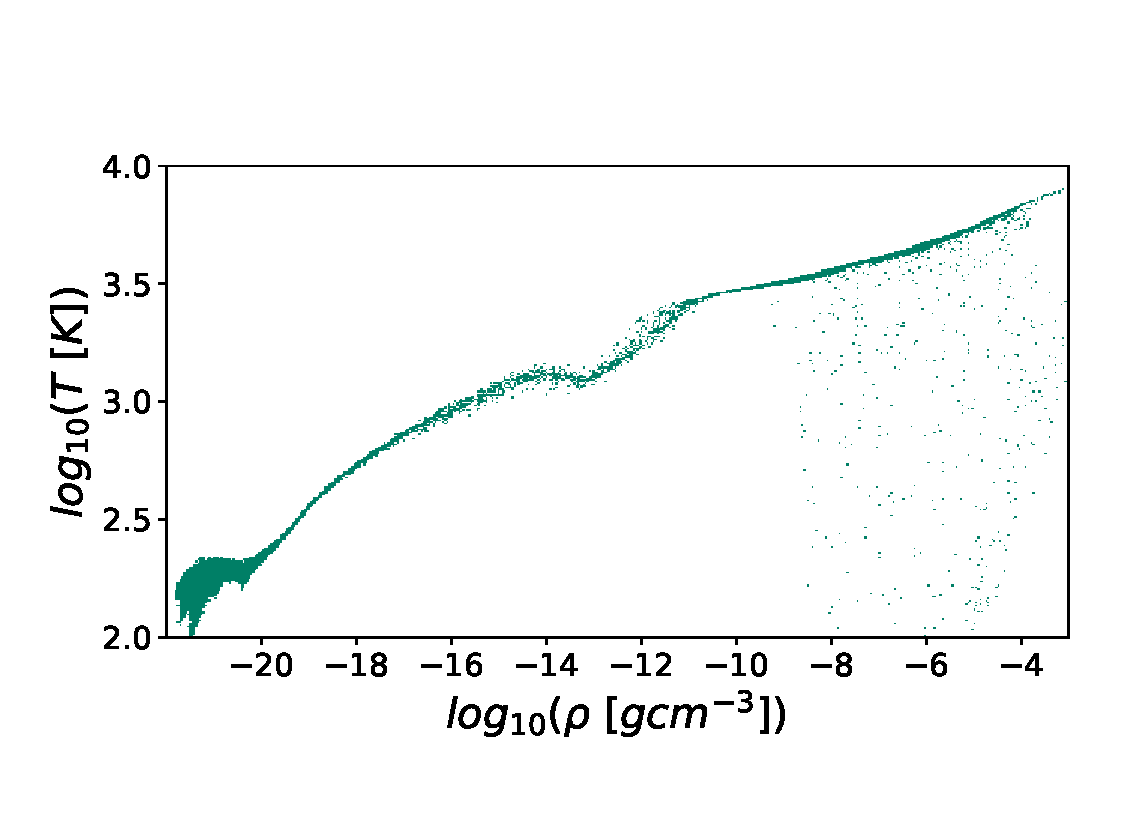
\includegraphics[scale=0.6]{simple.pdf}}
    \caption{Relationship between density and temperature during a collapse in the absence of turbulence, resulting in a single central dense object. As the computing time required is greater for pure collapse set-ups, the Jeans length was allowed to fall below the minimum cell size at at the highest densities, producing the artificial behaviour seen in the bottom right section of the figure.}
    \label{fig:simple}
\end{figure}

\begin{table}
	\centering
	\caption{Sink creation density, temperature, sink radius, minimum cell size and minimum gravitational softening lengths used in the study.}
	\label{table:1}
	\begin{tabular}{lcccr} % four columns, alignment for each
		\hline
		$\rho_{\text{sink}}$ [gcm$^{-3}$] & T [K] & $\lambda_J$ [cm] & $V_{\text{min}}$ [cm$^{3}$] & $L_{\text{soft}}$ [cm]\\
		\hline
		$10^{-10}$ & 3050 & 1.37$\times 10^{14}$ & 5.10$\times 10^{39}$ & 1.72$\times 10^{13}$\\
		$10^{-9}$ & 3350 & 4.56$\times 10^{13}$ & 1.86$\times 10^{38}$ & 5.70$\times 10^{12}$\\
		$10^{-8}$ & 3750 & 1.53$\times 10^{13}$ & 6.95$\times 10^{36}$ & 1.91$\times 10^{12}$\\
		$10^{-7}$ & 4100 & 5.05$\times 10^{12}$ & 2.51$\times 10^{35}$ & 6.31$\times 10^{11}$\\
		$10^{-6}$ & 4460 & 1.67$\times 10^{12}$  & 9.03$\times 10^{33}$ &  2.08$\times 10^{11}$\\
		\hline
	\end{tabular}
\end{table}





\section{Simulations}
\label{Sims}
Four iterations were performed with identical initial conditions, with the moving mesh code AREPO \citep{Springel2010}. The sink parameters were varied as given in table \ref{table:1}.  Additionally, the $\rho_{\text{sink}}$=10$^{-10}$gcm$^{-3}$ and 10$^{-7}$gcm$^{-3}$ runs were repeated while varying the Jeans refinements criteria from 8-32 cells per Jeans length. The initial conditions consist of a Bonner Ebert sphere, categorised by central density $n_c$=2$\times$10$^{-20}$ and radius R$_{\text{BE}}$=1.87pc. The sphere was placed in a box of side length 4R$_{\text{BE}}$ and the density was enhanced by a factor of 1.87 to promote collapse. A random velocity field was imposed on the box, generated from the turbulent power spectrum $\propto k^{-2}$. The rms velocity was scaled to give a ratio of kinetic to gravitation energy $\alpha$=0.05 and the initial box temperature was 200K. The simulations were performed with refinement criteria of 16 cells per Jeans length. The chemistry used was the same as \cite{Clark2011}, with abundances of H$_2$, H$^{+}$, D$^{+}$ and HD as x$_{\text{H}_{2}}$=10$^{-3}$, x$_{\text{H}^{+}}$=10$^{-7}$, $x_{\text{D}^{+}}$=2.6$\times$10$^{-12}$ and $x_{\text{HD}}$=3$\times$10$^{-7}$. The simulations include H$_2$ cooling, H$_{2}$ collisional dissociation cooling, H$_{2}$ destruction by charge transfer with H{\sc ii}, H$_{2}$ formation heating through H$^-$ ,H$_{2}^+$ and three-body H$_{2}$ formation , H{\sc i} collisional ionization cooling, He{\sc i} collisional ionization cooling, He{\sc ii} collisional ionization cooling, H{\sc ii} recombination cooling, Dielectronic and Radiative He{\sc ii} recombination cooling, He{\sc iii} recombination cooling, H$^{-}$ photodissociation heating, H$_{2}^+$ photodissociation heating, H{\sc i} photoionization heating, He{\sc i} photoionization heating, He{\sc ii}, photoionization heating, H$_2$ photoionization heating and H$^-$ formation cooling. The evolution of N$_{\text{sink}}$ and M$_{\text{total}}$ is shown in figure \ref{fig:sinks}.

\subsection{Sink mergers}
\cite{Bonnell2005} showed that massive stars can form through the merger of a high-mass close binary. The total number of sinks and their masses  would be unrepresentative of the IMF if they were allowed to bunch up and lie on top of one another without merging. Similarly to \cite{Federrath2010}, we allow sinks to merge if they fit four criteria: they lie within eachothers accretion radius, they are moving towards eachother $(\nabla \cdot v) < 0$, their accelerations give $(\nabla \cdot a) <0$ and they are gravitationally bound. Since sink particles carry no thermal data, the last criteria simply requires that their gravitational potential well exceeds the kinetic energy of the system. When the criteria are met, the larger of the sinks gains the mass and linear momentum of smaller sink, and its position is shifted to the center of mass of the system. We allow multiple mergers per time-step, based on mass hierarchy; if sink A is flagged to merge into sink B, and sink B is flagged to merge into sink C, then both A and B will be merged into sink C simultaneously. The resulting IMF at $\sim$400yrs is given in figure \ref{fig:IMF}, and the evolution of N$_{\text{sink}}$ and M$_{\text{total}}$ with time is shown in figure \ref{fig:sinks}. The resulting clusters are shown at different stages of collapse in figure \ref{fig:grid}. The total number of sinks formed, total mass in sinks, largest sink mass, number of sinks ejected from the system and number of mergers are given in table \ref{table:2}, at 400 and 1200yrs after the formation of the first sink.

% Example figure
\begin{figure}
	% To include a figure from a file named example.*
	% Allowable file formats are eps or ps if compiling using latex
	% or pdf, png, jpg if compiling using pdflatex
	 \hbox{\hspace{-1cm} 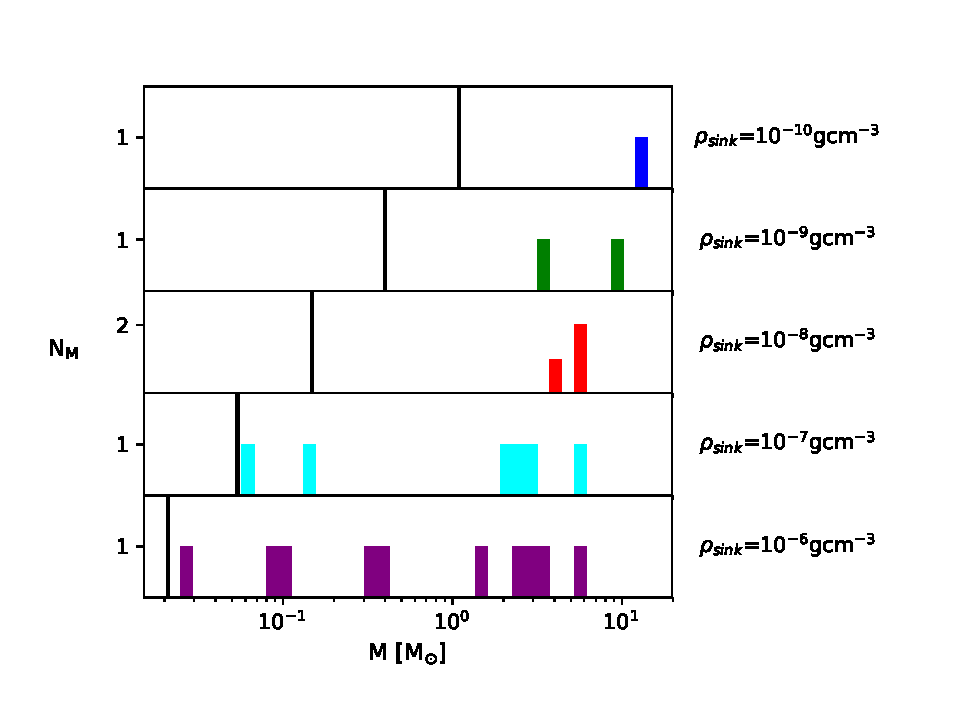
\includegraphics[scale=0.6]{IMF.pdf}}
    \caption{Initial mass functions taken at $t\sim$200 years after the formation of the first sink. The distribution of masses shifts towards lower masses with increasing $\rho_{\text{sink}}$. The minimum possible sink mass in each run is shown by a vertical black line, characterised by the sink radius and formation density. }
    \label{fig:IMF}
\end{figure}

% Example figure
\begin{figure*}
	% To include a figure from a file named example.*
	% Allowable file formats are eps or ps if compiling using latex
	% or pdf, png, jpg if compiling using pdflatex
	\hbox{\hspace{0cm} 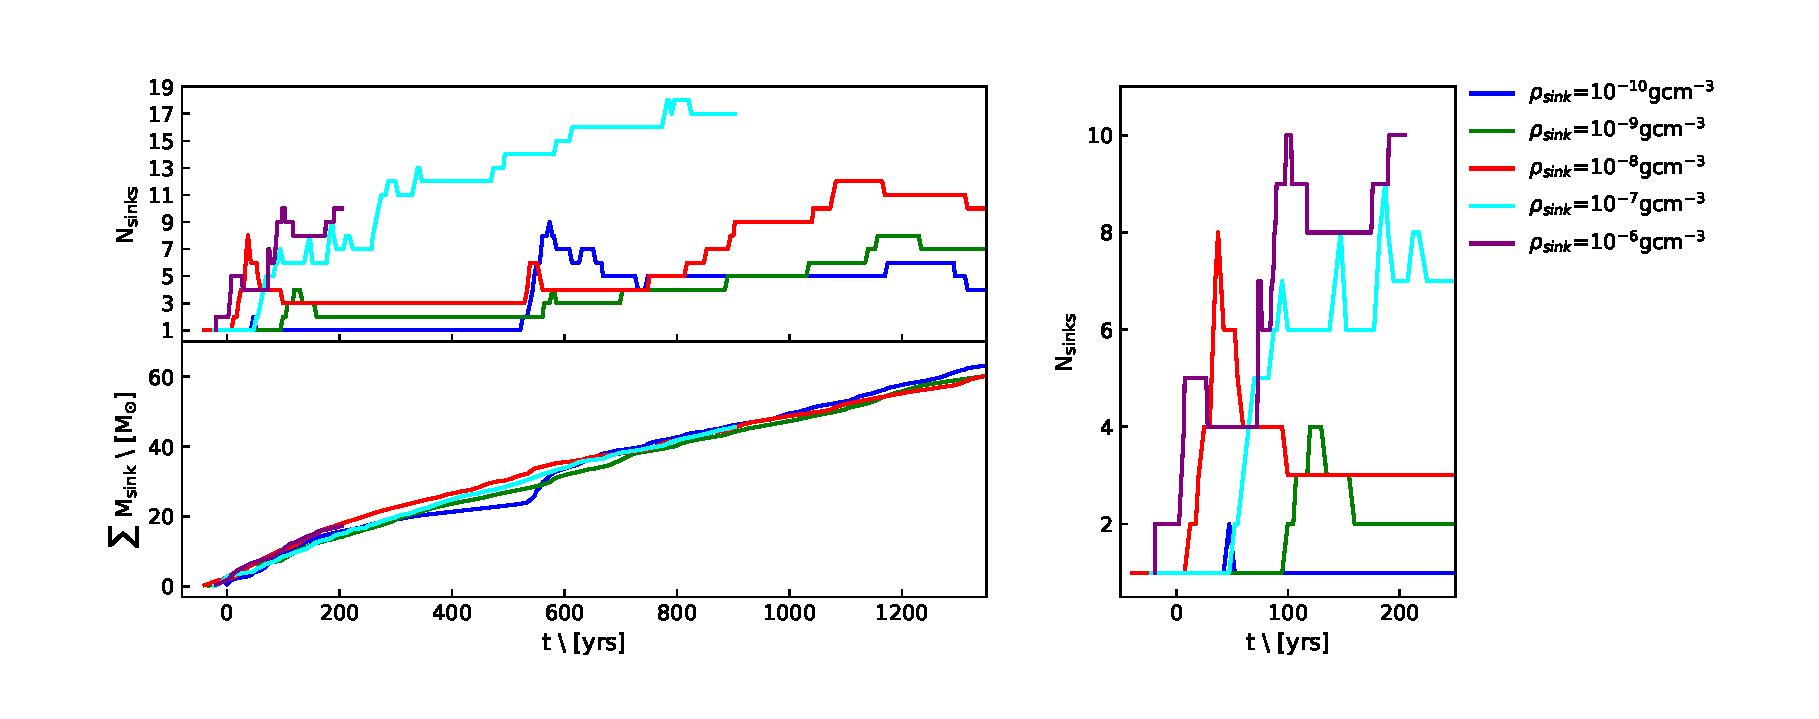
\includegraphics[scale=0.6]{sinks.pdf}}
    \caption{Evolution of the number of sinks and the total mass of all sinks with sink mergers enabled for $\rho_{\text{sink}}$=10$^{-10}$-10$^{-6}$gcm$^{-3}$. THe left hand panel shows the evolution of N$_{\text{sink}}$ zoomed into the first 250yrs.}
    \label{fig:sinks}
\end{figure*}

\begin{figure}

	 \hbox{\hspace{-1cm}  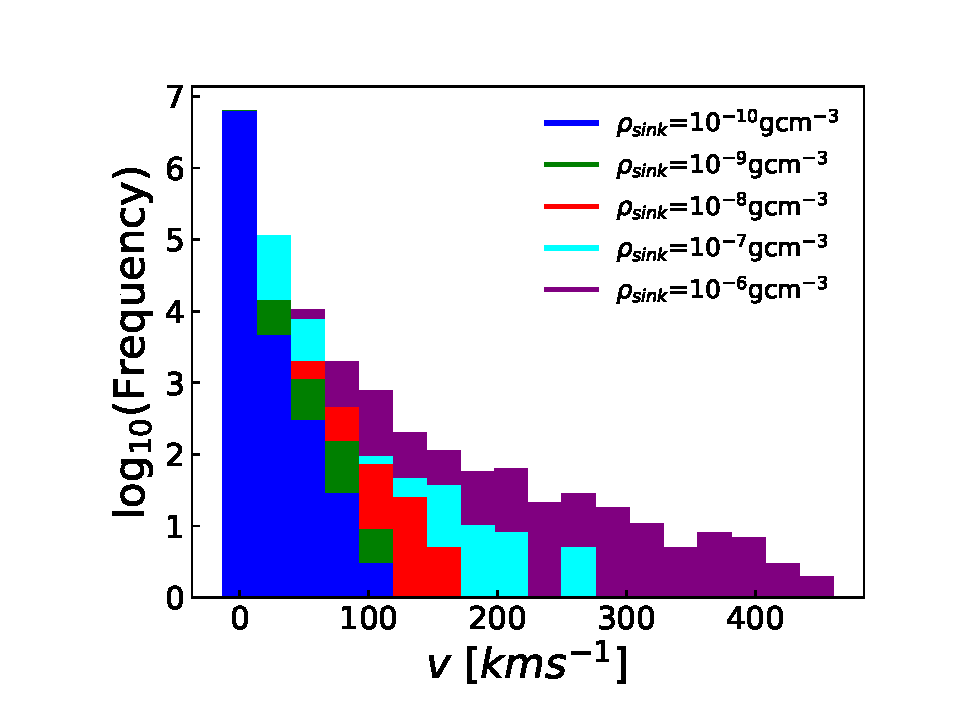
\includegraphics[scale=0.6]{velocities.pdf}}
    \caption{Cell velocity distributions for for $\rho_{\text{sink}}$=10$^{-10}$-10$^{-6}$gcm$^{-3}$ taken at $\sim$200yrs after the formation of the first sink.}
    \label{fig:cooling}
\end{figure}

\begin{figure}

	 \hbox{\hspace{-1cm}  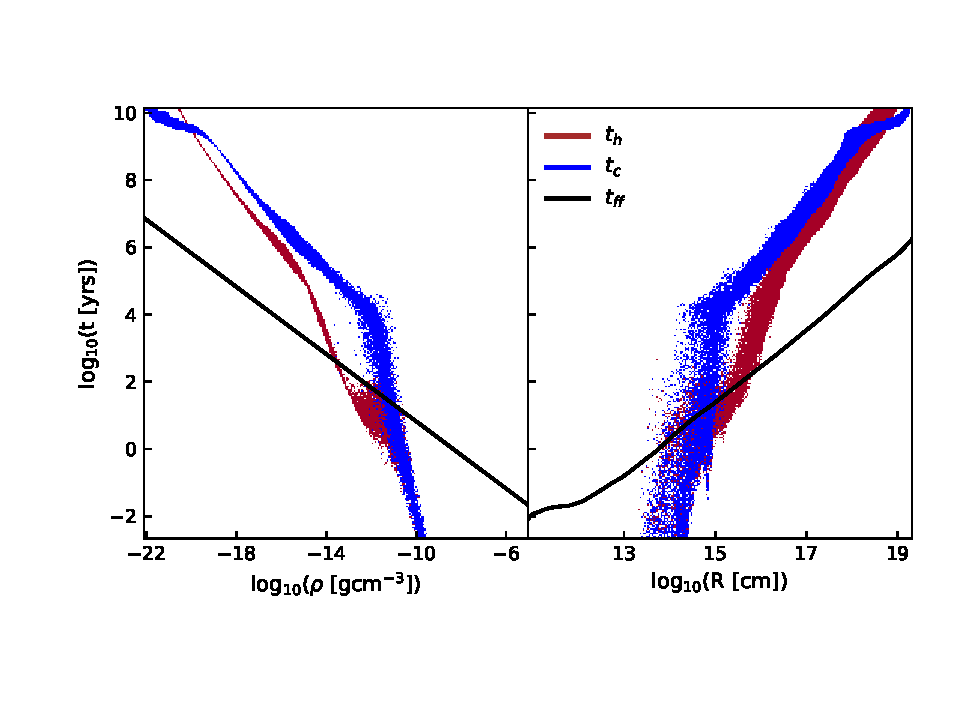
\includegraphics[scale=0.6]{cooling.pdf}}
    \caption{The chemical heating (red) and cooling (red) time-scales and free-fall time (black) as a function of density and radial distance.}
    \label{fig:cooling}
\end{figure}










\begin{table*}
	\centering
	\caption{The total number of sinks formed, total mass in sinks, largest sink mass, number of sinks ejected from the system and number of mergers at 400 and 1200yrs after the formation of the first sink.}
	\label{table:2}
	\begin{tabular}{l c c c | c c c | c c | c c c | c c| c c c |} % four columns, alignment for each
		\hline
		& &  & & t=200yrs & & & &  & t=400yrs & &  & &  &  t=1200yrs & \\
		\hline
		$\rho_{\text{sink}}$ & &  & N$_{\text{sink}}$ & M$_{\text{tot}}$ [M$_{\odot}$]  & N$_{\text{eject}}$& & &  N$_{\text{sink}}$ & M$_{\text{tot}}$ [M$_{\odot}$]  & N$_{\text{eject}}$ & & & N$_{\text{sink}}$ & M$_{\text{tot}}$ [M$_{\odot}$]   & N$_{\text{eject}}$  \\
		\hline
		$10^{-10}$ &&& 1 & 15.76 & 0 &&& 1  & 21.33 &   0    &&& 6  &  57.43    &  0   \\
		$10^{-9}$   &&& 2 & 14.20 & 0 &&& 2 & 23.63 &   0    &&& 8  &  55.59    &0   \\
		$10^{-8}$   &&& 3 & 17.93 & 0 &&& 3 & 26.59 &   0   &&&   11 &  55.28    &3    \\
		$10^{-7}$   &&& 7 & 15.14 & 1 &&&  12 & 25.39 &  5   &&& -  &  -            & $\geq$ 5   \\
		$10^{-6}$   &&& 10 & 17.18 & 1 &&&    -  &  -  & $\geq$ 1 &&& -& -& $\geq$ 1 \\
		\hline
	\end{tabular}
\end{table*}



 
\begin{figure*}
	% To include a figure from a file named example.*
	% Allowable file formats are eps or ps if compiling using latex
	% or pdf, png, jpg if compiling using pdflatex
	\hbox{\hspace{-0.5cm} 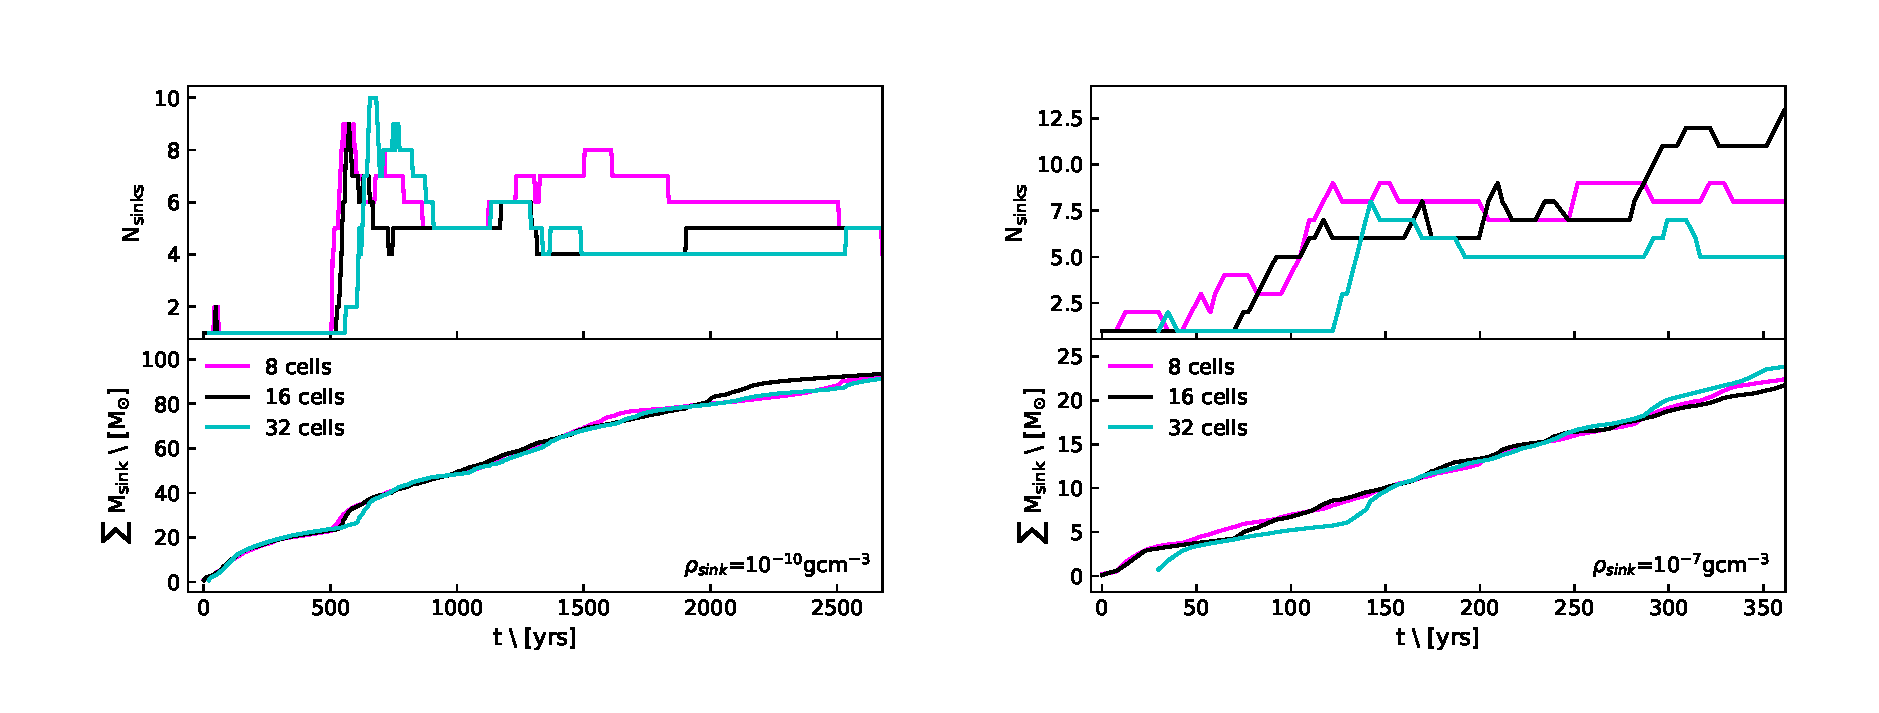
\includegraphics[scale=0.6]{jeans.pdf}}
    \caption{Evolution of the number of sinks and the total mass of all sinks with sink mergers enabled for $\rho_{\text{sink}}$=10$^{-10}$gcm$^{-3}$ and 10$^{-7}$gcm$^{-3}$, repeated with Jeans refinement criteria of 8, 16 and 32 cells per Jeans length.}
    \label{fig:jeans}
\end{figure*}



\section{Discussion}
\subsection{Sink morphology}
\label{study1}
Figure \ref{fig:sinks} shows that the total number of sinks formed did not converge within the range of sink formation densities used. Higher values of $\rho_{\text{sink}}$ gave higher number of sinks formed. The number of sinks formed, total mass in sinks, highest mass sink, number of ejected sinks, and number of sink mergers are given in table \ref{table:2}, at t=400yrs and t=1200yrs after the formation of the first sink. N$_{\text{sink}}$ may converge for higher $\rho_{\text{sink}}$ than tested in this study, but it is currently computationally impractical to run collapse problems to densities that high if the study attempts to cover a large parameter space such as turbulent energy or magnetic field strength. For the first $\sim$500yrs, the total mass in sinks also increased with increasing $\rho_{\text{sink}}$. However, after 600yrs, the total mass in sinks became invariant with changing sink parameters. As higher $\rho_{\text{sink}}$ produces higher N$_{\text{sink}}$ while M$_{\text{tot}}$ remains unaffected, using higher $\rho_{\text{sink}}$ produces lower mass stars and a broadened IMF. The mass of the largest sink in the group also decreased with increasing resolution. The resulting IMFs at time $t\sim$ 500yrs are given in figure \ref{fig:IMF}, the distribution of stars shifts towards lower mass populations with increasing $\rho_{\text{sink}}$. For the lowest resolution run, a single dense object forms in agreement with early numerical Pop III work (\citealt{Bromm1999}, \citealt{Haiman1996}), however it fragments into a broader IMF after $\sim$600yrs. Generally, the number of mergers increased with increasing resolution. The number of ejections from the group also increased with resolution. Due to the sink accretion radius decreasing with increasing $\rho_{\text{sink}}$, sinks had to be closer together before they could merge for higher $\rho_{\text{sink}}$ runs, possibly preventing mergers that could have kept the sinks from being ejected. The lower resolution rows of figure \ref{fig:grid} show the formation of disks and subsequent fragmentation in the early stages of collapse, that are absent in higher resolution runs. Unresolved, turbulent motions can produce artificial, large scale rotation \citep{Seifried2017}, to which these disks may be attributed. 



\subsection{Fragmentation instability}
The chemical heating and cooling time-scales ($t_h$ and $t_c$) were calculated by dividing cell internal energies by their total heating and cooling rates across all chemical processes, and are presented in figure \ref{fig:cooling}. Also shown is the cloud free-fall time, $t_{ff}$ given by 

\begin{equation}
t_{ff} = \sqrt{\frac{3\pi}{32G\rho_{\text{cloud}}}}
\end{equation}

Where $\rho_{\text{cloud}}$ is the mean density of the cloud. Cooling is balanced by chemical heating at densities above $\sim$10$^{-11}$gcm$^{-3}$. However, at $\sim$10$^{-6}$gcm$^{-3}$, the free-fall time exceeds the cooling time and effectively becomes the heating time-scale, allowing faster cooling than heating. Beyond this density, it could be said that the gas is unstable to fragmentation (e.g. the Gammie criterion). This density corresponds to a radius of 10$^{-13}$gcm$^{-3}$. The first simulation where sink particles were introduced at scales smaller than this was the $\rho_{\text{sink}}$=10$^{-11}$gcm$^{-3}$ run, which agrees with the jump in N$_{\text{sink}}$ seen in figure \ref{fig:sinks}. This suggests that $t_c < t_{ff}$ until the cooling from dissociation of H$_{2}$ molecules is depleted, where the collapse becomes almost adiabatic (stable to fragmentation). This means that the primordial IMF will not converge if sink particles are introduced before H$_{2}$ is depleted at 10$^{-4}$gcm$^{-3}$. The implications of this are that all previous studies using sink particles in primordial star formation have underestimated the number of Pop III objects forming in the halo, and have produced IMFs with higher mass stars than what would be achieved running without sink particles.


% Example figure
\begin{figure*}
	% To include a figure from a file named example.*
	% Allowable file formats are eps or ps if compiling using latex
	% or pdf, png, jpg if compiling using pdflatex
	\hbox{\hspace{-2cm} 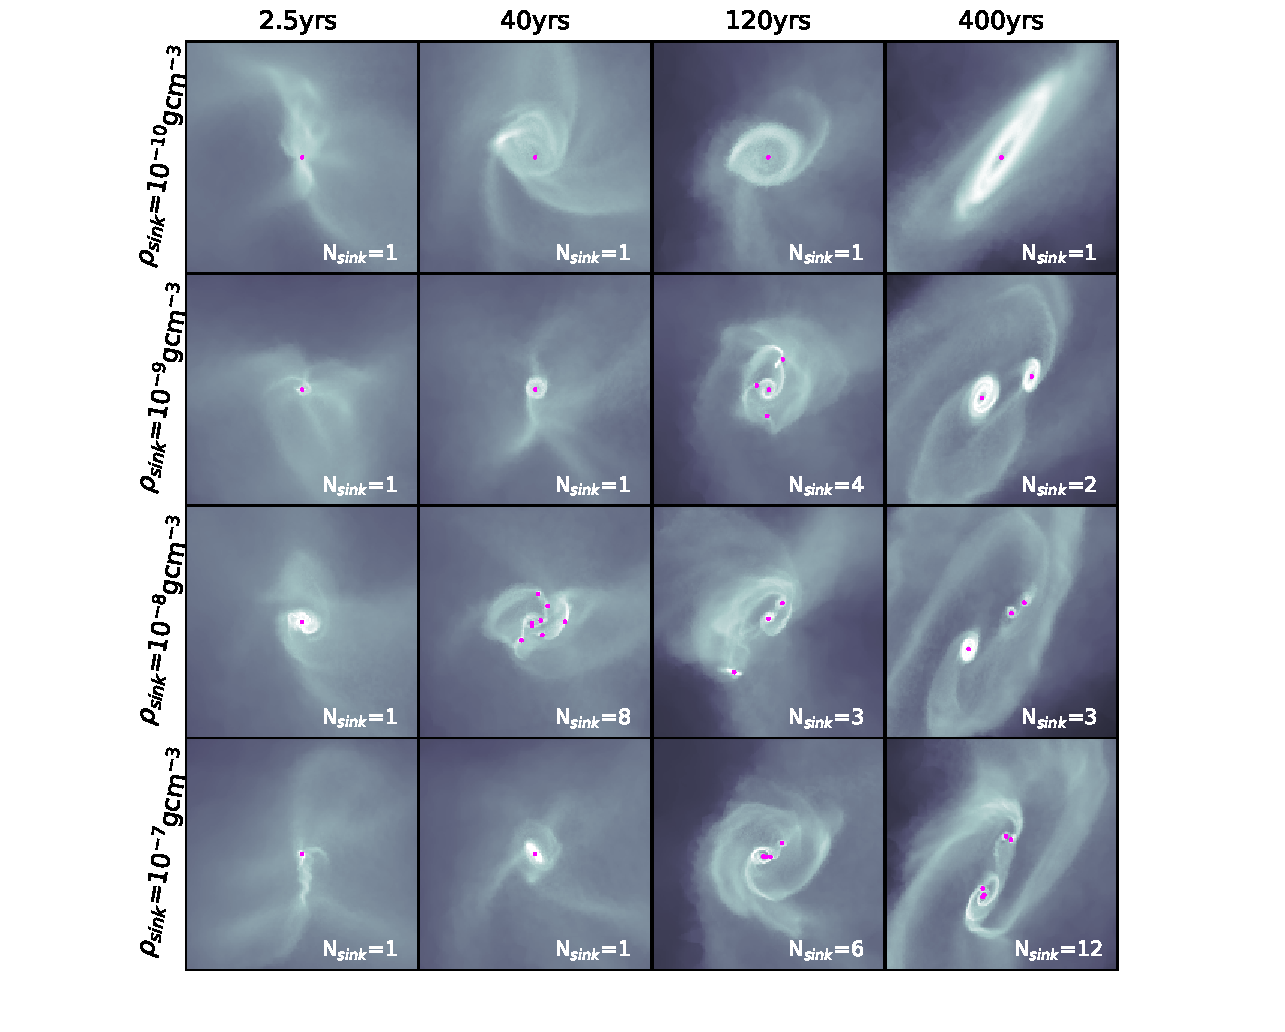
\includegraphics[scale=1]{grid1.pdf}}
    \caption{Density plots taken at 2.5, 40, 120 and 400 years after the formation of the first sink particle. A, B, C and D correspond to $\rho_{\text{sink}}$=$10^{-10}$,$10^{-9}$, $10^{-8}$ and $10^{-7}$gcm$^{-3}$. Sink particles are shown as red dots. The box lengths shown are all of side length 107AU. The simulations were performed with sink mergers enabled.}
    \label{fig:grid}
\end{figure*}

\subsection{Jeans refinement criteria}
The simulations discussed in section \ref{study1} were performed with a Jeans refinement criteria of 16 cells per Jeans length during the collapse. \cite{Truelove1997} found that at least 4 cells per Jeans length necessary, but not  sufficient  for convergence in isothermal self-gravitational hydrodynamics problems. An authors choice refinement criteria becomes particularly important in magnetised collapses, as higher refinement results in greater amplification of the magnetic field (e.g. \citealt{Federrath2011,Turk2012}). Figure \ref{fig:jeans} shows the variation of N$_{\text{sink}}$ and M$_{\text{sink}}$ when choosing 8, 16 or 32 cells per Jeans length. The initial fragmentation of the central object is delayed when using higher Jeans criteria. Although the  evolution of N$_{\text{sink}}$ follows the same general shape across each run, the subsequent value of N$_{\text{sink}}$ at any point after the initial burst of star formation is stochastic and doesn't suggest any correlation between resolution criteria and final IMF. Once again, the accretion rate and total mass in sinks is unaffected by refinement criteria. N-body problems are chaotic; small differences between runs are expected to change the results somewhat. In this case, the differences caused by varying refinement criteria have caused variation in N$_{\text{sink}}$, but it is reassuring that no clear trend becomes apparent within the range tested. These results suggest that 8 cells per Jeans length is sufficient to prevent artificial fragmentation in hydrodynamic problems. In magneto-hydrodynamic (MHD) problems, however, magnetic fields support against gas fragmentation, resulting in a reduction of low-mass stars \citep{Sharda2020}. This means that using higher refinement criteria would reduce N$_{\text{sink}}$ in MHD set-ups.

\section{Conclusions}

In a Population III setting, the effect of varying the sink particle creation density was investigated. A turbulent cloud collapse resulting in periodic brsts of star formation was repeated for sink creation densities spanning the range $10^{-10}$-$10^{-6}$gcm$^{-3}$. It was found that higher sink creation densities result in a larger number of sinks formed without converging within the range tested. The total mass in sinks is was independent of the sink parameters used, resulting in an IMF that shifts towards lower mass stars with higher sink creation density. The IMF, however, does converge when sinks are introduced at $10^{-7}$gcm$^{-3}$ or higher. The cooling time-scale becomes smaller than the free-fall time at $\sim 10^{-6}$gcm$^{-3}$, resulting in instability to fragmentation and enhanced numbers of sinks forming when sink particles are creates beyond this density. It is expected that the cooling time-scale will increase once the H$_2$ is completely dissociated at 10$^{-4}$gcm$^{-3}$, creating stability. The number of sink mergers and ejections from the system increased with increasing sink creation density, due to the higher velocities achieved as $\rho_{\text{sink}}$ increased. The effects of Jeans refinement criteria were also investigated, with higher Jeans criteria resulting in delayed fragmentation of the central object, but stochastic evolutions of N$_{\text{sink}}$. The accretion rates onto sinks were also unaffected by Jeans refinement criteria.

\section*{Acknowledgements}



%%%%%%%%%%%%%%%%%%%%%%%%%%%%%%%%%%%%%%%%%%%%%%%%%%


 





%%%%%%%%%%%%%%%%%%%% REFERENCES %%%%%%%%%%%%%%%%%%

% The best way to enter references is to use BibTeX:
\newpage
\bibliographystyle{mnras}

\bibliography{references.bib} % if your bibtex file is called example.bib



%%%%%%%%%%%%%%%%%%%%%%%%%%%%%%%%%%%%%%%%%%%%%%%%%%

%%%%%%%%%%%%%%%%% APPENDICES %%%%%%%%%%%%%%%%%%%%%




%%%%%%%%%%%%%%%%%%%%%%%%%%%%%%%%%%%%%%%%%%%%%%%%%%


% Don't change these lines
\bsp	% typesetting comment
\label{lastpage}

\end{document}

% End of mnras_template.tex